\documentclass[tikz,border=2pt]{standalone}
\usepackage{amsmath}
\usepackage{pgfplots}
\pgfplotsset{compat=1.18}
\usetikzlibrary{arrows.meta}
\begin{document}
% a = 100, b = 1, c = 10: follower's best response q2 = (90 - q1)/2. The leader picks the point
% on BR_2 with the highest profit: her iso-profit curve v_1 = 1012.5, i.e. q2 = 90 - q1 - 1012.5/q1,
% is tangent to BR_2 at (45, 22.5). The Cournot point (30, 30) also lies on BR_2 (leader profit 900).
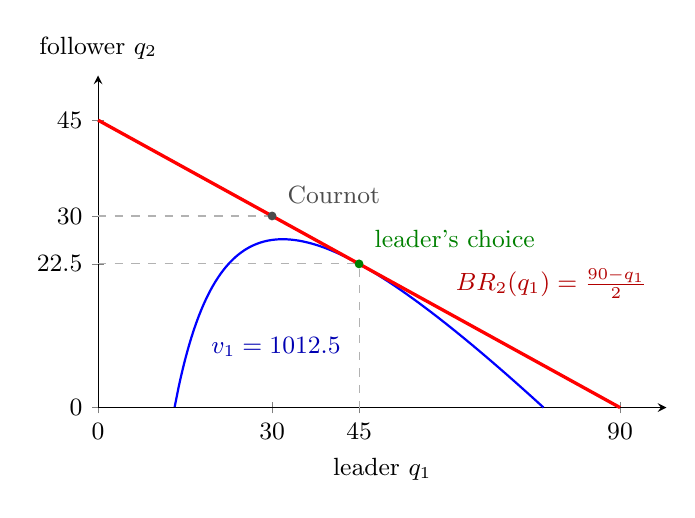
\begin{tikzpicture}[font=\small, >={Latex[length=2mm]}]
  \begin{axis}[
    axis lines=left, xmin=0, xmax=98, ymin=0, ymax=52,
    xtick={0,30,45,90}, ytick={0,22.5,30,45},
    xlabel={leader $q_1$}, ylabel={follower $q_2$},
    ylabel style={rotate=-90, anchor=south, at={(axis description cs:0,1.02)}},
    width=8.8cm, height=5.8cm, clip=false]
    \addplot[gray!60, thin, dashed] coordinates {(0,22.5) (45,22.5) (45,0)};
    \addplot[gray!60, thin, dashed] coordinates {(0,30) (30,30)};
    \addplot[blue, thick, domain=13.2:76.8, samples=80, smooth] {90-x-1012.5/x};
    \addplot[red, very thick, domain=0:90, samples=2] {(90-x)/2};
    \fill[gray!60!black] (axis cs:30,30) circle (1.6pt);
    \fill[green!50!black] (axis cs:45,22.5) circle (1.6pt);
    \node[red!70!black, anchor=south west] at (axis cs:60,15.5) {$BR_2(q_1)=\frac{90-q_1}{2}$};
    \node[gray!60!black, anchor=south west] at (axis cs:31,30.5) {Cournot};
    \node[green!50!black, anchor=south west] at (axis cs:46,23.5) {leader's choice};
    \node[blue!70!black, anchor=north east] at (axis cs:43.5,12.5) {$v_1=1012.5$};
  \end{axis}
\end{tikzpicture}
\end{document}
